\documentclass[10.5pt,a4paper]{article}

\usepackage[utf8]{inputenc}
\usepackage[T1]{fontenc}
\usepackage{lmodern}
\usepackage[portuguese]{babel}
\usepackage[margin=2.2cm]{geometry}
\usepackage{amsmath}
\usepackage{booktabs}
\usepackage{array}
\usepackage{graphicx}
\usepackage{caption}
\usepackage{subcaption}
\usepackage{enumitem}
\usepackage{listings}
\usepackage{pgfplots}
\usepackage[colorlinks=true,linkcolor=black,citecolor=black,urlcolor=blue]{hyperref}

\pgfplotsset{compat=1.16}
\captionsetup{font=small,labelfont=bf}
\setlist[itemize]{itemsep=2pt,topsep=4pt}
\setlength{\parskip}{3pt}
\renewcommand{\arraystretch}{1.12}

\lstset{
  basicstyle=\ttfamily\scriptsize,
  breaklines=true,
  breakatwhitespace=false,
  columns=fullflexible,
  keepspaces=true,
  frame=single,
  framerule=0.3pt,
  xleftmargin=2pt,
  xrightmargin=2pt,
  upquote=true
}

\newcommand{\ip}[1]{\texttt{#1}}

\title{\textbf{Análise e Redução do Volume de Tráfego do FACEIT (CS2):\\
Captura Global, Classificação, Filtragem e Agregação em Fluxos}}
\author{\textbf{GRUPO 6}\\[2pt]
Ivo Costa Sousa -- pg63976\\
João Afonso Almeida Sousa -- pg62405\\
João Carlos Teixeira Neiva -- pg63978}
\date{Novembro de 2026}

\begin{document}
\maketitle

\begin{abstract}
\noindent Este relatório, desenvolvido para a Unidade Curricular de Qualidade de Serviço na
Internet, analisa o tráfego gerado pela plataforma FACEIT durante uma partida de CS2. A partir
de uma captura global com o Wireshark (326\,122 pacotes, 206,9~MB, cerca de 30 minutos), o
serviço é classificado num plano de jogo (um único fluxo UDP, 79\,\% dos bytes, sem marcação
DSCP e com um pacote a cada 15,6~ms) e num plano de controlo (DNS, TLS e QUIC, cerca de 2\,\%
dos bytes). São estudados os critérios de filtragem mais eficazes e quantificada a redução de
volume obtida por filtragem (21,3\,\%), truncagem de pacotes (87,5\,\%), \emph{sampling}
combinado com truncagem (98,9\,\%) e agregação em fluxos com o Argus e com o tshark
(99,97\,\% e 99,96\,\%, respetivamente).
\end{abstract}

%% ------------------------------------------------------------------
\section{Parte 1: Objetivos e Metodologia}

\subsection{Objetivos}
Este trabalho consolida as etapas estudadas sobre captura e análise de tráfego, tendo como
serviço de estudo o FACEIT, plataforma competitiva de partidas de CS2 que exige a execução de
um cliente de \emph{Anti-Cheat} próprio~\cite{faceitac}. Os objetivos definidos foram:
\begin{itemize}
  \item \textbf{Captura global:} gerar tráfego real do serviço e capturar todo o tráfego da
        máquina com o Wireshark~\cite{wireshark}.
  \item \textbf{Classificação e filtragem:} estudar os critérios mais eficazes, tanto em
        filtros de captura como em filtros de visualização.
  \item \textbf{Redução de volume:} quantificar a percentagem de otimização face à captura
        global por filtragem, truncagem de pacotes e \emph{sampling}.
  \item \textbf{Agregação em fluxos:} explorar ferramentas de agregação de pacotes em fluxos
        a partir de ficheiros pcap.
\end{itemize}

\subsection{Captura}
O Wireshark correu na própria máquina de jogo (\ip{192.168.1.82}), ligada por cabo, sem filtro
de captura e com pacotes inteiros, durante 1\,818,6~s (cerca de 30 minutos) e com o FACEIT
\emph{Anti-Cheat} ativo. Antes da captura final realizou-se um ensaio num servidor normal de
CS2, fora do FACEIT, para validar o procedimento.

\subsection{Estratégia de Análise}
Optou-se por uma única captura global, convertida para pcap simples (\texttt{editcap -F pcap})
para servir de \emph{baseline}. Todos os cenários reduzidos foram derivados \emph{offline}
desse mesmo ficheiro, garantindo que a comparação incide exatamente sobre o mesmo tráfego.
Recorreu-se ao Wireshark/tshark, editcap, capinfos, tcpdump e ao Argus~\cite{argus}. A
percentagem de otimização foi calculada, em bytes (tamanho do ficheiro) e em número de
pacotes, por:
\[
  \text{redução} = \left(1 - \frac{\text{tamanho reduzido}}{\text{tamanho global}}\right)\times 100.
\]
O tamanho do ficheiro inclui 16~B de cabeçalho por pacote no formato pcap. O campo
\emph{Data size} do capinfos não reflete a truncagem, pelo que não foi utilizado.

%% ------------------------------------------------------------------
\section{Parte 2: Caracterização do Tráfego}

\subsection{Visão Geral}\label{sec:visao}
A captura global contém 326\,122 pacotes e 201,6~MB de dados (212,6~MB em pcapng e 206,9~MB em
pcap), com uma média de 618~B por pacote e 179 pacotes/s. A composição por classe encontra-se
na Tabela~\ref{tab:comp}; as classes sobrepõem-se parcialmente, pelo que não devem ser somadas.

\begin{table}[htbp]
\centering
\caption{Composição do tráfego global.}\label{tab:comp}
\small
\begin{tabular}{@{}lrrrr@{}}
\toprule
Classe & Pacotes & Bytes & \% Pacotes & \% Bytes\\
\midrule
Servidor de jogo (\ip{141.95.32.214})      & 202\,086 & 159\,679\,469 & 62,0 & 79,2\\
UDP :19336 (\ip{104.29.146.69})            &  85\,785 &  17\,938\,347 & 26,3 &  8,9\\
TCP (todo)                                 &  19\,394 &  12\,376\,258 &  5,9 &  6,1\\
QUIC (todo)                                &   7\,226 &   9\,622\,529 &  2,2 &  4,8\\
mDNS / SSDP / DNS                          &   4\,576 &   1\,307\,245 &  1,4 &  0,6\\
Controlo FACEIT (\ip{193.41.200.101/102})  &   3\,995 &   3\,338\,873 &  1,2 &  1,7\\
\bottomrule
\end{tabular}
\end{table}

A primeira linha conta todos os pacotes com o IP do servidor (202\,086), incluindo 80 que não
pertencem à conversa UDP principal (202\,006 pacotes, o valor usado no resto do relatório).
Estes 80 pacotes são ICMP (Figura~\ref{fig:trace}) e correspondem a um \emph{traceroute}
(Secção~\ref{sec:aux}).

\begin{figure}[htbp]
\centering
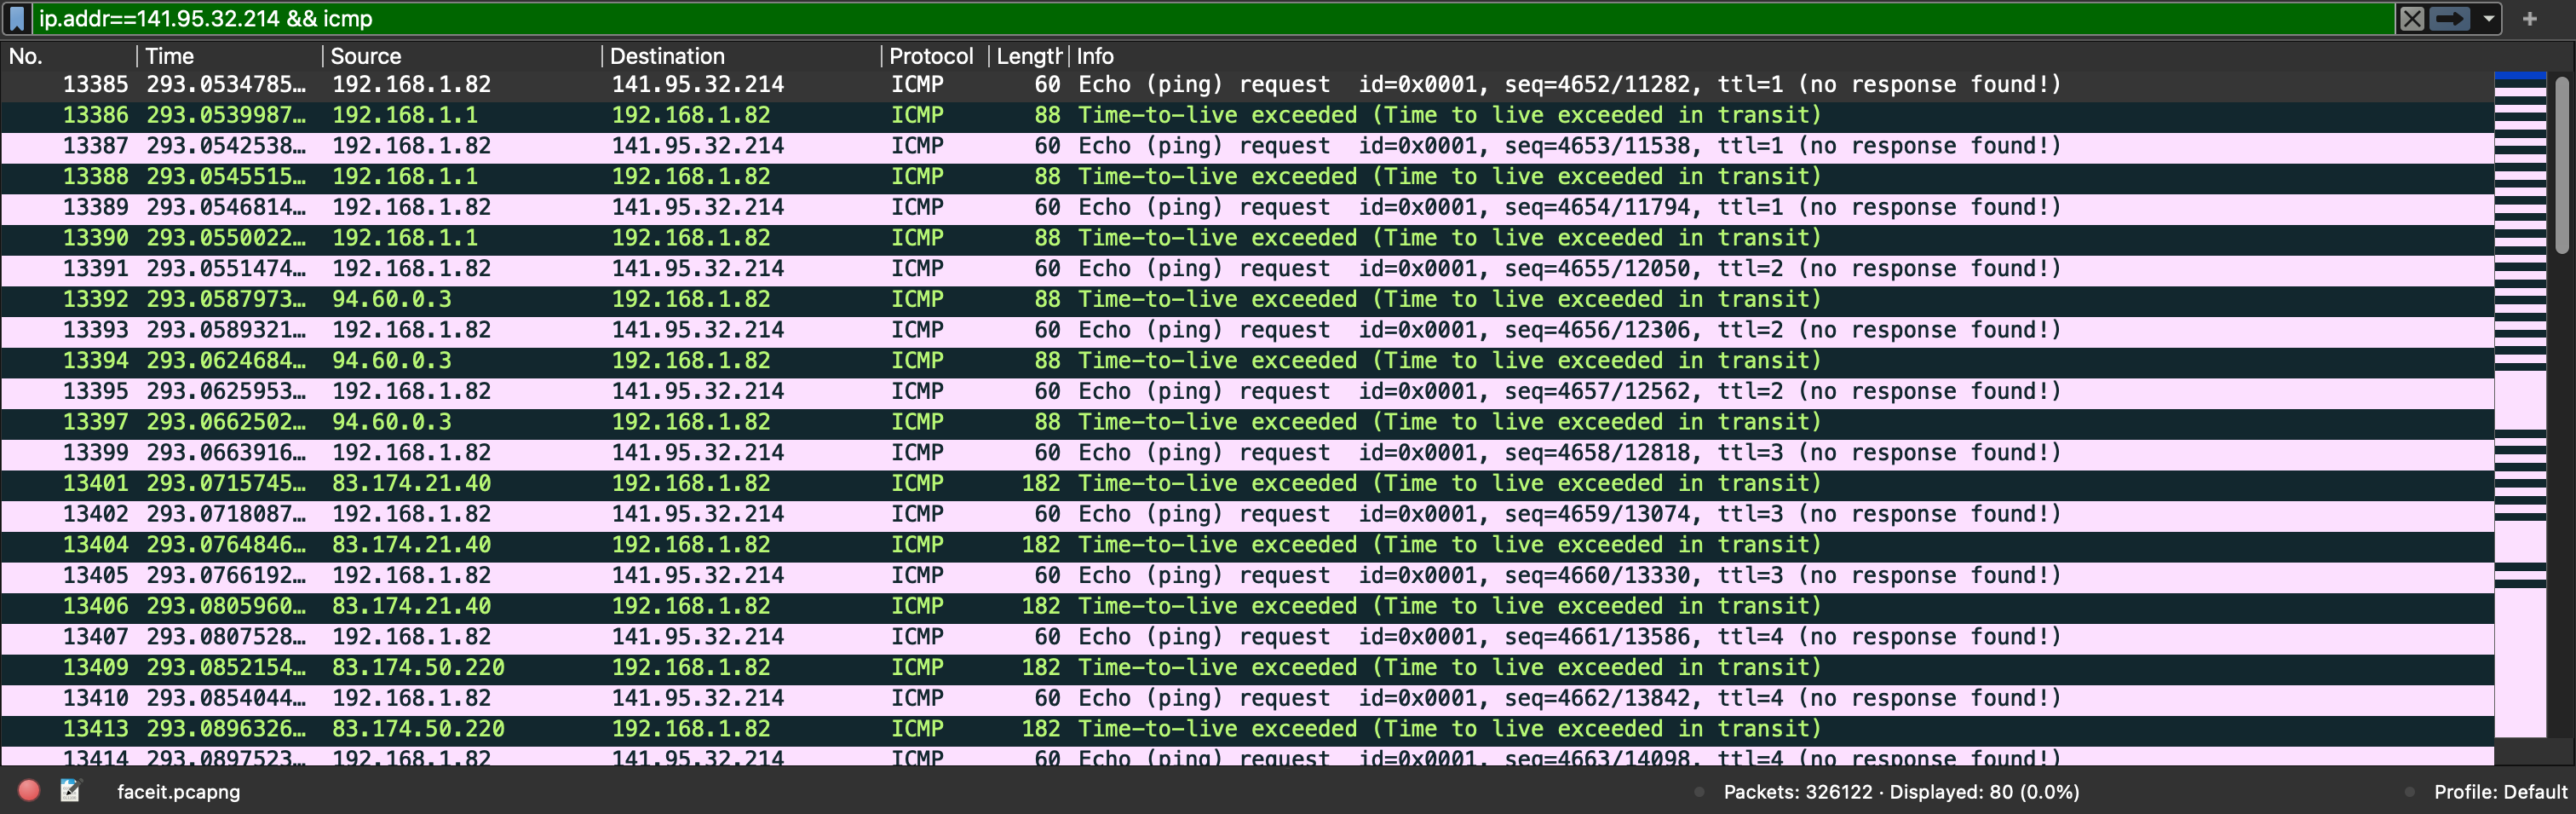
\includegraphics[width=\textwidth]{figs/fig_icmp80.png}
\caption{Filtro \texttt{ip.addr==141.95.32.214 \&\& icmp}: os 80 pacotes ICMP com o IP do
servidor, ou seja, sondas com TTL crescente e respostas \emph{Time-to-live exceeded} dos
\emph{routers} intermédios.}\label{fig:trace}
\end{figure}

\subsection{Plano de Jogo}
A conversa UDP \ip{192.168.1.82:50088} $\leftrightarrow$ \ip{141.95.32.214:27031} domina a
captura (Figura~\ref{fig:conv}). Inicia-se aos 293,8~s, dura 1\,520,5~s e totaliza 202\,006
pacotes e 159,7~MB. Os seus principais indicadores são:
\begin{itemize}
  \item \textbf{Cliente $\to$ servidor:} 96\,786 pacotes (70,7~MB), com média de 730~B por pacote.
  \item \textbf{Servidor $\to$ cliente:} 105\,220 pacotes (89,0~MB), com média de 846~B por pacote.
  \item \textbf{Débito:} praticamente constante, com cerca de 133 pacotes/s e 0,84~Mbit/s
        (aproximadamente 40\,000 pacotes por cada 300~s).
  \item \textbf{Tamanho dos pacotes:} concentrado entre 640 e 1\,279~B (69,3\,\% dos pacotes),
        com média de 790~B.
\end{itemize}

\begin{figure}[htbp]
\centering
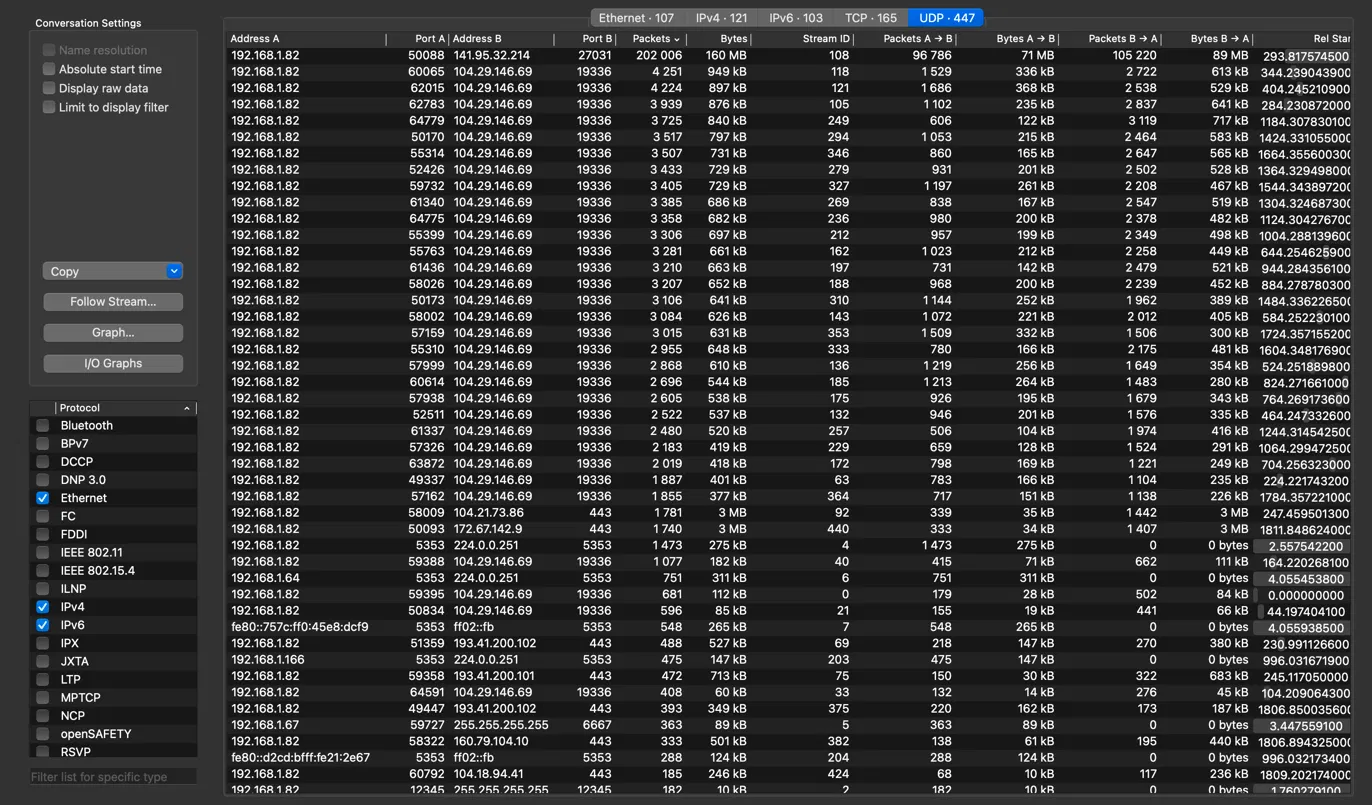
\includegraphics[width=0.92\textwidth]{figs/fig1.png}
\caption{\emph{Conversations} $\to$ UDP, ordenado por pacotes: o fluxo para
\ip{141.95.32.214:27031} domina.}\label{fig:conv}
\end{figure}

\subsection{Características de QoS do Fluxo de Jogo}
Como a Unidade Curricular se centra na Qualidade de Serviço, caracterizou-se o fluxo de jogo do
ponto de vista da marcação e da regularidade temporal, medidas no ponto de captura (a máquina de
jogo). Os 202\,006 pacotes têm DSCP~0 nos dois sentidos, ou seja, o tráfego é tratado como
\emph{best effort}, sem qualquer marcação de QoS. A Tabela~\ref{tab:ipt} resume o tempo entre
pacotes consecutivos de cada sentido. Neste relatório, o \emph{jitter} é medido pelo
desvio-padrão desse tempo (7,58~ms no sentido servidor $\to$ cliente e 4,02~ms no sentido
inverso).

\begin{table}[htbp]
\centering
\caption{Tempo entre pacotes consecutivos do fluxo de jogo (ms).}\label{tab:ipt}
\small
\begin{tabular}{@{}lrrrrrrr@{}}
\toprule
Sentido & Pacotes & Média & Mediana & p95 & p99 & Máximo & Desvio-padrão\\
\midrule
Servidor $\to$ cliente & 105\,220 & 14,45 & 15,60 & 16,05 & 16,52 & 1\,000,4 & 7,58\\
Cliente $\to$ servidor &  96\,786 & 15,71 & 15,64 & 16,65 & 17,11 &    518,6 & 4,02\\
\bottomrule
\end{tabular}
\end{table}

As medianas de cerca de 15,6~ms correspondem a aproximadamente 64 pacotes/s por sentido, e os
percentis 95 e 99 ficam muito próximos da mediana, o que mostra um fluxo muito regular. No
sentido servidor $\to$ cliente, a média abaixo da mediana e o desvio-padrão maior sugerem
pacotes que chegam em rajadas, e os máximos de 1\,000~ms e 519~ms correspondem a interrupções
isoladas. Trata-se, portanto, de um fluxo de baixo débito mas sensível à latência e ao
\emph{jitter}.

\subsection{Plano de Controlo}
O DNS e o SNI (em TLS e QUIC) permitem identificar inequivocamente o serviço
(Figura~\ref{fig:ctrl}). Foram observados os nomes \texttt{www.faceit.com},
\texttt{edge.faceit.com}, \texttt{chat.faceit.com}, \texttt{faceit.com},
\texttt{cdn-frontend.faceit-cdn.net}, \texttt{distribution.faceit-cdn.net} e
\texttt{ac-client-ws.faceit.com}, todos resolvidos para \ip{193.41.200.101} e
\ip{193.41.200.102}, a que se junta \texttt{analytics.faceitanalytics.com} (Cloudflare). O
primeiro contacto ocorre aos 2,2~s (QUIC para \texttt{www.faceit.com}), surge uma nova rajada de
pedidos entre os 225 e os 245~s, antes de o fluxo de jogo começar, e um último contacto a
\texttt{ac-client-ws.faceit.com} aos 1\,804,6~s. Este plano é reduzido: 3\,995 pacotes e
3,3~MB (1,7\,\% dos bytes).

\begin{figure}[htbp]
\centering
\begin{subfigure}{\textwidth}
  \centering
  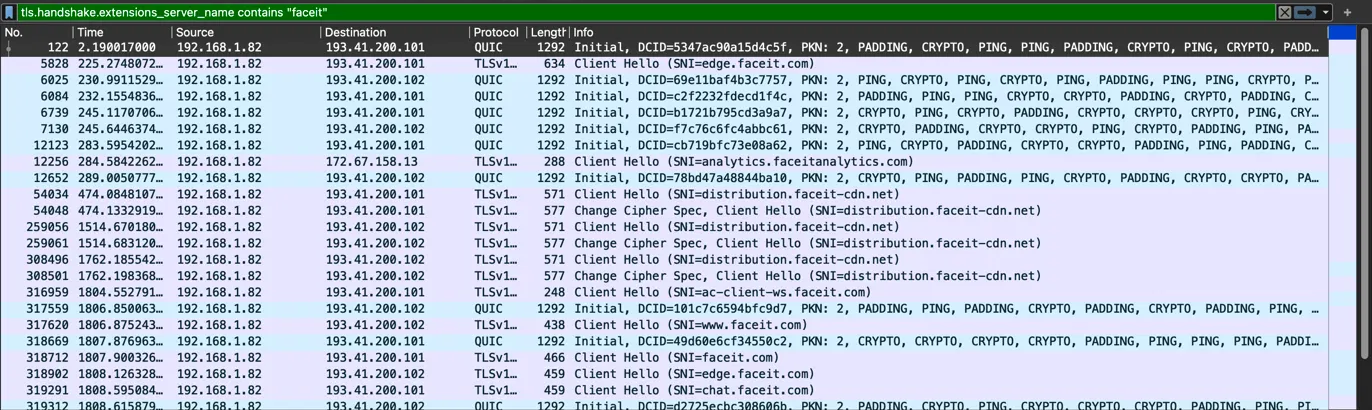
\includegraphics[width=\textwidth]{figs/fig2.png}
  \caption{\texttt{tls.handshake.extensions\_server\_name contains "faceit"} (TLS e QUIC).}
\end{subfigure}\\[4pt]
\begin{subfigure}{\textwidth}
  \centering
  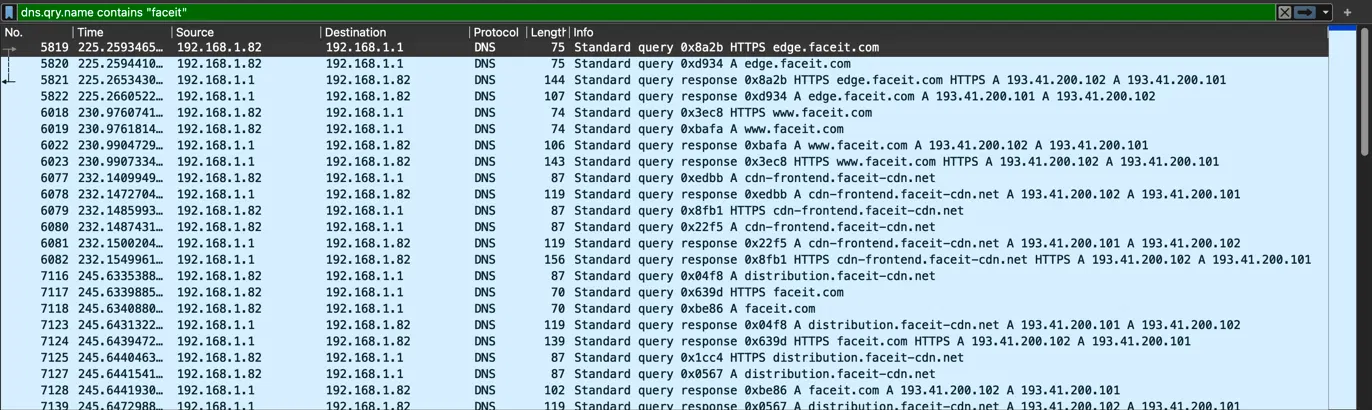
\includegraphics[width=\textwidth]{figs/fig3.png}
  \caption{\texttt{dns.qry.name contains "faceit"}.}
\end{subfigure}
\caption{Identificação do plano de controlo por filtros de visualização.}\label{fig:ctrl}
\end{figure}

\subsection{Tráfego Auxiliar e Ruído}\label{sec:aux}
\textbf{Traceroute.} Aos 293,05~s, pouco antes de o fluxo UDP começar, o cliente envia 51
\emph{Echo requests} ICMP para o servidor, com TTL de 1 a 17 (três sondas por TTL) e o texto
\texttt{icmp-trace-packet} no \emph{payload}, ou seja, um \emph{traceroute}
(Figura~\ref{fig:trace}, na Secção~\ref{sec:visao}). Recebe 26 mensagens \emph{Time-to-live exceeded} de nove \emph{routers}
intermédios (os saltos 7, 8 e 11 não respondem) e 3 \emph{Echo replies} do próprio servidor, no
salto 17. Os 51 + 26 + 3 = 80 pacotes são exatamente os que distinguem os 202\,086 da
Tabela~\ref{tab:comp} dos 202\,006 da conversa UDP. Não foi confirmado qual o processo que o
gera (possivelmente o cliente do jogo).

As respostas permitem estimar o RTT até ao servidor, \emph{a priori} um valor indicativo, já que
os \emph{routers} geram ICMP com baixa prioridade: cerca de 0,4~ms no primeiro salto (\emph{router}
doméstico), 3,6~ms no segundo, 4--5~ms nos saltos 3 e 4, 29~ms no salto 5 e cerca de 55,7~ms
até ao servidor (média das três \emph{Echo replies}).

\textbf{Ruído.} Os fluxos UDP para \ip{104.29.146.69:19336} (um novo fluxo por minuto, 85\,785
pacotes) são independentes do jogo, uma vez que surgiam também na captura de ensaio; a sua
origem não foi identificada. Há ainda uma ligação TCP de longa duração (1\,818~s) para
\ip{185.25.182.20:27021}, provavelmente do cliente Steam, e tráfego da rede local (mDNS, SSDP,
\emph{broadcasts}) e outras ligações HTTPS/QUIC.

%% ------------------------------------------------------------------
\section{Parte 3: Critérios de Classificação e Filtragem}

\subsection{Filtros Estudados}
O filtro de captura (BPF)~\cite{pcapfilter} apenas tem acesso aos cabeçalhos (IP, protocolo,
portas), pelo que critérios baseados em nomes (DNS/SNI) só são possíveis como filtros de
visualização. A eficácia de cada critério foi avaliada através da \textbf{cobertura} (pacotes do
jogo apanhados / pacotes do jogo) e da \textbf{precisão} (pacotes do jogo apanhados / pacotes
apanhados), tomando como referência a conversa do jogo (202\,006 pacotes). Os resultados constam
da Tabela~\ref{tab:filtros}.

\begin{table}[htbp]
\centering
\caption{Critérios de classificação e respetiva eficácia.}\label{tab:filtros}
\footnotesize
\begin{tabular}{@{}>{\raggedright\arraybackslash}p{2.3cm}
                  >{\raggedright\arraybackslash\ttfamily}p{3.9cm}
                  >{\raggedright\arraybackslash\ttfamily}p{4.5cm}
                  r r@{}}
\toprule
\rmfamily Critério & \rmfamily Filtro de captura (BPF) & \rmfamily Filtro de visualização &
\rmfamily Pacotes & \rmfamily Precisão\\
\midrule
\rmfamily Servidor (IP) & udp and host 141.95.32.214 & ip.addr==141.95.32.214 \&\& udp &
\rmfamily 202\,006 & \rmfamily 100\,\%\\
\rmfamily Qualquer protocolo com o IP & host 141.95.32.214 & ip.addr==141.95.32.214 &
\rmfamily 202\,060 & \rmfamily 99,97\,\%\\
\rmfamily Gama de portas & udp portrange 27000-27050 & udp.port>=27000 \&\& udp.port<=27050 &
\rmfamily 202\,040 & \rmfamily 99,98\,\%\\
\rmfamily Só UDP & udp & udp & \rmfamily 300\,571 & \rmfamily 67,2\,\%\\
\rmfamily Controlo (IP) & host 193.41.200.101 or host 193.41.200.102 &
ip.addr==193.41.200.101 || ip.addr==193.41.200.102 & \rmfamily 3\,995 & \rmfamily ---\\
\rmfamily Controlo (nome) & \rmfamily (não aplicável) &
dns.qry.name contains "faceit"; tls.handshake.extensions\_server\_name contains "faceit" &
\rmfamily --- & \rmfamily ---\\
\rmfamily Jogo + controlo (IPs) & host servidor or host controlo (2 IPs) & --- &
\rmfamily 206\,055 & \rmfamily ---\\
\rmfamily Portas + controlo & udp portrange 27000-27050 or host 193.41.200.101 or host 193.41.200.102 &
--- & \rmfamily 206\,035 & \rmfamily ---\\
\bottomrule
\end{tabular}
\end{table}

\subsection{Discussão}
Todos os filtros baseados em IP ou em portas atingem uma cobertura de 100\,\% do fluxo de jogo. A
gama de portas apanha apenas 34 pacotes a mais do que o filtro por IP (precisão de 99,98\,\%) e
tem a vantagem de não depender do IP do servidor, que muda de partida para partida. Em
contrapartida, o filtro apenas por protocolo (\texttt{udp}) revela-se demasiado abrangente, já
que 33\,\% do que apanha não pertence ao jogo.

O filtro BPF \texttt{host 141.95.32.214} apanha 202\,060 pacotes, ou seja, mais 54 do que a
conversa UDP: são as 51 sondas e as 3 respostas do \emph{traceroute}. O filtro de visualização
\texttt{ip.addr==141.95.32.214} chega aos 202\,086 da Tabela~\ref{tab:comp} porque o Wireshark
também compara o IP do pacote original embebido nas 26 mensagens \emph{Time-to-live exceeded},
que o BPF (que só olha para o cabeçalho exterior) não vê. Os filtros que incluem \texttt{udp}
deixam este \emph{traceroute} de fora, o que é aceitável para o estudo do jogo.

Conclui-se que a deteção do fluxo de jogo é mais eficaz através da combinação de três critérios:
transporte UDP, gama de portas 27xxx e dominância por volume (\emph{Conversations} ordenado por
bytes), sendo o serviço confirmado pelo DNS/SNI do plano de controlo. Para uma captura ao vivo,
em que o IP do servidor ainda não é conhecido, o filtro mais adequado é o último da
Tabela~\ref{tab:filtros}, que junta a gama de portas aos dois IPs do plano de controlo.

%% ------------------------------------------------------------------
\section{Parte 4: Redução de Volume}

\subsection{Resultados}
A Tabela~\ref{tab:red} e a Figura~\ref{fig:red} apresentam os cenários avaliados. Todas as
percentagens são calculadas face ao \emph{baseline} (A) de 326\,122 pacotes e 206\,864\,624~B.

\begin{table}[htbp]
\centering
\caption{Redução de volume face à captura global.}\label{tab:red}
\small
\begin{tabular}{@{}llrrrr@{}}
\toprule
 & Cenário & Pacotes & Bytes & Red.\ bytes & Red.\ pacotes\\
\midrule
A  & Captura global (\emph{baseline})                      & 326\,122 & 206\,864\,624 & 0\,\%     & 0\,\%\\
B1 & Filtro \texttt{udp and host} servidor                 & 202\,006 & 162\,905\,309 & 21,25\,\% & 38,06\,\%\\
B3 & Filtro gama de portas 27000--27050                    & 202\,040 & 162\,951\,481 & 21,23\,\% & 38,05\,\%\\
B4 & Filtro só \texttt{udp}                                & 300\,571 & 193\,613\,964 &  6,41\,\% &  7,83\,\%\\
B5 & Filtro jogo + controlo FACEIT (IPs)                   & 206\,055 & 166\,312\,206 & 19,60\,\% & 36,82\,\%\\
B6 & Filtro portas + controlo FACEIT                       & 206\,035 & 166\,354\,274 & 19,58\,\% & 36,82\,\%\\
C1 & B1 + \emph{snaplen} 128                               & 202\,006 &  32\,311\,732 & 84,38\,\% & 38,06\,\%\\
C2 & B1 + \emph{snaplen} 96                                & 202\,006 &  25\,856\,584 & 87,50\,\% & 38,06\,\%\\
C3 & B1 + \emph{snaplen} 64                                & 202\,006 &  19\,392\,644 & 90,63\,\% & 38,06\,\%\\
C4 & B5 + \emph{snaplen} 96                                & 206\,055 &  26\,333\,772 & 87,27\,\% & 36,82\,\%\\
C5 & B6 + \emph{snaplen} 96 (filtro recomendado)           & 206\,035 &  26\,333\,156 & 87,27\,\% & 36,82\,\%\\
D1 & B1 + \emph{sampling} 1/10                             &  20\,200 &  16\,376\,628 & 92,08\,\% & 93,81\,\%\\
D2 & B1 + \emph{snaplen} 96 + \emph{sampling} 1/10         &  20\,200 &   2\,262\,424 & 98,91\,\% & 93,81\,\%\\
E1 & Fluxos Argus, global (registos de 5~s)                & --- &  1\,004\,872 & 99,51\,\% & ---\\
E2 & Fluxos Argus, global (1 registo/fluxo, CSV)           & --- &     64\,839 & 99,97\,\% & ---\\
E3 & Fluxos Argus, só servidor (CSV, 1 fluxo)              & --- &        229 & $\approx$100\,\% & ---\\
E4 & Conversas tshark, global (texto, UDP+TCP)             & --- &     89\,824 & 99,96\,\% & ---\\
\bottomrule
\end{tabular}
\end{table}

\begin{figure}[htbp]
\centering
\begin{tikzpicture}
\begin{axis}[
  xbar,
  width=0.92\textwidth,
  height=8.6cm,
  xmin=0, xmax=112,
  xlabel={Redução face à captura global (\% dos bytes)},
  symbolic y coords={B1 filtro IP,B3 filtro portas,B6 portas+controlo,C1 snaplen 128,C2 snaplen 96,C3 snaplen 64,C5 filtro recomendado,D1 sampling 1/10,D2 snaplen 96 + sampling,E1 Argus 5 s,E4 tshark conversas,E2 Argus 1/fluxo},
  ytick=data,
  y dir=reverse,
  bar width=7pt,
  enlarge y limits=0.05,
  tick label style={font=\scriptsize},
  label style={font=\small},
  nodes near coords={\pgfmathprintnumber[fixed,fixed zerofill,precision=2,use comma]{\pgfplotspointmeta}},
  nodes near coords align={horizontal},
  every node near coord/.append style={font=\scriptsize},
  xmajorgrids=true,
  grid style={gray!25}
]
\addplot[fill=blue!55!black!70,draw=none] coordinates {
  (21.25,B1 filtro IP) (21.23,B3 filtro portas) (19.58,B6 portas+controlo)
  (84.38,C1 snaplen 128) (87.50,C2 snaplen 96) (90.63,C3 snaplen 64)
  (87.27,C5 filtro recomendado) (92.08,D1 sampling 1/10)
  (98.91,D2 snaplen 96 + sampling) (99.51,E1 Argus 5 s)
  (99.96,E4 tshark conversas) (99.97,E2 Argus 1/fluxo)
};
\end{axis}
\end{tikzpicture}
\caption{Redução de bytes por cenário.}\label{fig:red}
\end{figure}

\subsection{Filtragem}
Filtrar o fluxo de jogo reduz apenas 21,25\,\% dos bytes, mas 38,06\,\% dos pacotes. Esta
assimetria explica-se pelo facto de o jogo já representar 79\,\% dos bytes capturados, enquanto
o ruído é composto por muitos pacotes pequenos: os 85\,785 pacotes de \texttt{:19336}
correspondem a 26\,\% dos pacotes, mas a apenas 9\,\% dos bytes. Incluir o plano de controlo no
filtro tem um custo reduzido (19,58\,\% a 19,60\,\% contra 21,25\,\%) e descreve o serviço de
forma mais completa.

\subsection{Truncagem de Pacotes (Snaplen)}
Não capturar o pacote inteiro é a técnica com maior impacto individual. Os cabeçalhos Ethernet,
IPv4 e UDP ocupam 42~B, pelo que, com \emph{snaplen} 96, se preservam os cabeçalhos e mais 54~B
de \emph{payload}. Com pacotes de 790~B em média, a redução total sobe de 21,25\,\% para
87,50\,\% (84,38\,\% com 128~B e 90,63\,\% com 64~B). O custo é a perda do restante
\emph{payload}.

\subsection{Sampling}
Guardar 1 pacote em cada 10 (por ordem de pacote) proporciona uma redução de 92,08\,\% sem
truncagem e de 98,91\,\% com \emph{snaplen} 96 (2,26~MB, dos quais cerca de 0,32~MB
correspondem a cabeçalhos de pacote do formato pcap). As estatísticas de volume mantêm-se
fiáveis: extrapolando $\times$10, o erro é de $-0{,}003$\,\% nos pacotes e de $+0{,}54$\,\% nos
bytes. Perdem-se, contudo, as sequências de pacotes consecutivos.

\subsection{Impacto nas Métricas de QoS}
As técnicas não são equivalentes para quem quer medir QoS. A filtragem e o \emph{snaplen} 96
mantêm todos os pacotes, as marcas temporais e o cabeçalho IP (onde está o DSCP), pelo que ainda
permitem calcular o tempo entre pacotes e o \emph{jitter} da Tabela~\ref{tab:ipt}. O
\emph{sampling} 1/10 preserva volumes e distribuições de tamanhos, mas os intervalos medidos
entre pacotes amostrados deixam de corresponder aos reais. A agregação em fluxos conserva o
débito médio e a duração, mas perde o \emph{jitter}.

%% ------------------------------------------------------------------
\section{Parte 5: Agregação de Pacotes em Fluxos}

\subsection{Ferramentas e Processo}
Exploraram-se duas ferramentas sobre o mesmo \texttt{A\_global.pcap}. O Argus
(\texttt{argus -r f.pcap -w f.argus}) emite registos de estado de cerca de 5~s por fluxo, e o
\texttt{racluster} agrupa-os num único registo por fluxo (5-tuplo), exportado para CSV através do
\texttt{ra}. O tshark produz, com \texttt{-z conv,udp -z conv,tcp}, uma lista de conversas UDP e
TCP em texto.

\subsection{Resultados}
A Tabela~\ref{tab:agg} compara as saídas obtidas a partir do \emph{baseline} de 206,9~MB.

\begin{table}[htbp]
\centering
\caption{Agregação em fluxos: Argus e tshark.}\label{tab:agg}
\small
\begin{tabular}{@{}lrrrl@{}}
\toprule
Saída & Registos & Tamanho (B) & Redução & Protocolos\\
\midrule
Argus, registos de 5~s (binário)    & ---  & 1\,004\,872 & 99,51\,\% & todos\\
Argus, 1 registo por fluxo (binário) & 797 &    122\,656 & 99,94\,\% & todos\\
Argus, 1 registo por fluxo (CSV)    & 797  &     64\,839 & 99,97\,\% & todos\\
tshark conversas (texto)            & 612  &     89\,824 & 99,96\,\% & UDP e TCP\\
\bottomrule
\end{tabular}
\end{table}

As duas ferramentas chegam a ordens de grandeza semelhantes (cerca de 65~kB a 90~kB, mais de
99,9\,\%), mas diferem no que registam:
\begin{itemize}
  \item \textbf{Cobertura de protocolos:} o tshark só lista UDP e TCP (447 e 165 conversas, tal
        como mostram os separadores das \emph{Conversations}). O Argus regista também ICMPv6,
        ARP, IGMP, ICMP e LLDP, daí os 797 fluxos (mais um registo de gestão do Argus), dos
        quais cerca de 200 não são UDP nem TCP.
  \item \textbf{Fluxos TCP:} o Argus tem 149 fluxos TCP e o tshark 165. Na captura existem 149
        5-tuplos TCP distintos, que é o que o \texttt{racluster} agrega. A diferença de 16
        conversas vem de quatro ligações a \ip{192.168.1.166:8009} (porta tipicamente usada
        por dispositivos Google Cast na rede local) que repetem o mesmo 5-tuplo cinco vezes: o
        tshark conta cada nova tentativa de ligação como uma conversa distinta, o Argus junta-as
        num único registo ($4\times 4 = 16$). Isto significa que o Argus agrega por 5-tuplo e o
        tshark por ligação.
  \item \textbf{Precisão dos totais:} o tshark em texto arredonda os bytes (por exemplo,
        159~MB para o fluxo de jogo), enquanto o Argus conserva os valores exatos.
\end{itemize}

Os totais do fluxo de jogo no Argus (70\,661\,525~B do cliente e 89\,011\,664~B do servidor)
somam 159\,673\,189~B, exatamente o volume de dados do pcap filtrado. Aplicado ao filtro do
servidor, o fluxo de jogo fica reduzido a um único registo de 229~B no CSV. A agregação conserva
o 5-tuplo, o instante de início, a duração e os pacotes e bytes por sentido, mas perde a
temporização e o tamanho de cada pacote, bem como o \emph{payload}. Os registos de 5~s do Argus
conservam ainda a evolução temporal do fluxo.

%% ------------------------------------------------------------------
\section{Parte 6: Conclusões}

\subsection{Síntese}
\begin{itemize}
  \item \textbf{Estrutura do serviço:} plano de jogo (UDP \ip{141.95.32.214:27031}, 79\,\% dos
        bytes) e plano de controlo (DNS/TLS/QUIC para \ip{193.41.200.101/102}, 1,7\,\% dos bytes).
  \item \textbf{Classificação:} os critérios mais eficazes para detetar o fluxo de jogo são o
        transporte UDP, a gama de portas 27000--27050 e a dominância por volume; o DNS/SNI
        confirma o serviço. O filtro apenas por protocolo é demasiado abrangente.
  \item \textbf{QoS do fluxo de jogo:} DSCP~0 em todos os pacotes, um pacote a cada 15,6~ms em
        cada sentido com pouco desvio, e um RTT até ao servidor de cerca de 56~ms.
  \item \textbf{Redução de volume:} a filtragem poupa pouco em bytes (21\,\%), dado que o jogo
        domina a captura. As maiores poupanças resultam do \emph{snaplen} (87,5\,\%), do
        \emph{sampling} (98,9\,\% em conjunto) e da agregação em fluxos (99,5\,\% a 99,97\,\%).
  \item \textbf{Escolha da técnica:} depende da utilização pretendida: cabeçalhos e tempos por
        pacote $\Rightarrow$ filtro e \emph{snaplen} 96; estatísticas de volume $\Rightarrow$
        \emph{sampling}; contabilização e retenção prolongada $\Rightarrow$ fluxos.
\end{itemize}

\subsection{Configuração de Captura Recomendada}
Para uma captura ao vivo deste serviço recomenda-se o filtro de portas e IPs de controlo com
\emph{snaplen} 96, por exemplo com o \texttt{dumpcap}:
\begin{lstlisting}
dumpcap -i <n> -f "udp portrange 27000-27050 or host 193.41.200.101 or host 193.41.200.102" -s 96 -w captura.pcapng
\end{lstlisting}
Aplicada \emph{offline} à captura global, esta configuração (C5) guarda 206\,035 pacotes em
26,3~MB, uma redução de 87,27\,\% dos bytes, e mantém os cabeçalhos, as marcas temporais e as
\emph{queries} DNS (70 a 87~B, que cabem inteiras). Em contrapartida, as respostas DNS (até
156~B) ficam truncadas e o SNI deixa de ser legível: no TLS surge para lá dos 96~B do pacote e,
nos QUIC \emph{Initial} (1\,292~B), só se obtém decifrando o pacote completo. Com este
\emph{snaplen}, o plano de controlo é portanto identificado pelos IPs e não pelo nome do
serviço. Esta configuração não foi validada numa captura ao vivo.

\subsection{Limitações}
Foi analisada uma única captura de uma única partida, e o IP e a porta do servidor mudam entre
partidas, pelo que a gama de portas 27000--27050 pode não se aplicar a outros servidores. Os
cenários foram derivados \emph{offline} da captura global, e não capturados ao vivo. O
\emph{sampling} aplicado é determinístico (1 em 10 por ordem de pacote) e as percentagens em
ficheiro incluem o cabeçalho de 16~B por pacote do formato pcap. O tempo entre pacotes e o RTT
foram medidos no ponto de captura e incluem, por isso, o efeito da rede e do próprio sistema de
captura. A agregação em fluxos usou apenas o Argus e o tshark.

%% ------------------------------------------------------------------
\begin{thebibliography}{9}\small
\bibitem{wireshark} Wireshark Foundation, \emph{Wireshark User's Guide}.
  \url{https://www.wireshark.org/docs/wsug_html_chunked/}
\bibitem{pcapfilter} The Tcpdump Group, \emph{pcap-filter(7) --- packet filter syntax}.
  \url{https://www.tcpdump.org/manpages/pcap-filter.7.html}
\bibitem{argus} QoSient, \emph{Argus --- Auditing Network Activity}. \url{https://openargus.org}
\bibitem{faceitac} FACEIT, \emph{What is FACEIT Anti-cheat and how does it work?}
  \url{https://support.faceit.com/hc/en-us/articles/9394666828188-What-is-FACEIT-Anti-cheat-and-how-does-it-work}
\end{thebibliography}

%% ------------------------------------------------------------------
\appendix
\section{Comandos Utilizados}
\begin{lstlisting}
# Baseline
capinfos faceit.pcapng
editcap -F pcap faceit.pcapng A_global.pcap

# Caracterizacao
tshark -r A_global.pcap -q -z io,phs
tshark -r A_global.pcap -q -z conv,udp
tshark -r A_global.pcap -q -z plen,tree,"ip.addr==141.95.32.214"
tshark -r A_global.pcap -Y 'dns.flags.response==1 && dns.qry.name contains "faceit"' -T fields -e frame.time_relative -e dns.qry.name -e dns.a
tshark -r A_global.pcap -Y 'tls.handshake.extensions_server_name contains "faceit"' -T fields -e frame.time_relative -e ip.dst -e tls.handshake.extensions_server_name

# Traceroute (80 pacotes ICMP com o IP do servidor fora da conversa UDP)
tshark -r A_global.pcap -Y "ip.addr==141.95.32.214 && icmp" -q -z io,phs
tshark -r A_global.pcap -Y "icmp && ip.addr==141.95.32.214" -T fields -e frame.time_relative -e ip.src -e ip.ttl -e icmp.type -e icmp.seq_le
# RTT por salto: emparelhamento das sondas com as respostas pelo numero de sequencia (Python)

# QoS do fluxo de jogo (DSCP e instantes; os intervalos foram calculados em Python)
tshark -r B1_udp_host.pcap -T fields -e ip.dsfield.dscp | sort | uniq -c
tshark -r B1_udp_host.pcap -Y "ip.src==141.95.32.214" -T fields -e frame.time_epoch

# Filtros (BPF, aplicados offline)
tcpdump -r A_global.pcap -w B1_udp_host.pcap "udp and host 141.95.32.214"
tcpdump -r A_global.pcap -w B3_portrange.pcap "udp portrange 27000-27050"
tcpdump -r A_global.pcap -w B4_udp.pcap "udp"
tcpdump -r A_global.pcap -w B5_game_ctrl.pcap "host 141.95.32.214 or host 193.41.200.101 or host 193.41.200.102"
tcpdump -r A_global.pcap -w B6_portrange_ctrl.pcap "udp portrange 27000-27050 or host 193.41.200.101 or host 193.41.200.102"

# Snaplen e sampling
editcap -s 96 B1_udp_host.pcap C2_snaplen96.pcap
editcap -s 96 B6_portrange_ctrl.pcap C5_portrange_ctrl_snaplen96.pcap
tshark -r C2_snaplen96.pcap -Y "frame.number % 10 == 0" -F pcap -w D2_snaplen_sampling.pcap

# Fluxos (Argus)
argus -r A_global.pcap -w E1_global.argus
racluster -r E1_global.argus -m proto saddr sport daddr dport -w E2_global_cluster.argus
ra -r E2_global_cluster.argus -n -c , -s stime dur proto saddr sport daddr dport spkts dpkts sbytes dbytes > E2_global_flows.csv

# Fluxos (tshark) e medicao
tshark -r A_global.pcap -q -z conv,udp -z conv,tcp > flows_tshark.txt
capinfos -T -m -M -c -s *.pcap
\end{lstlisting}

\end{document}
